\documentclass[a4paper,12pt]{scrreprt}

\usepackage[italian]{babel}

\usepackage[utf8]{inputenc}

\usepackage{mathtools}
\DeclarePairedDelimiter{\ceil}{\lceil}{\rceil}

\usepackage{graphicx}
\graphicspath{{images/}}

\usepackage{tcolorbox}
\tcbuselibrary{theorems,minted,breakable}
\newtcbtheorem[number within=chapter]{mynote}{Nota}{%
  colback=blue!5,
  colframe=blue!35!black,
  breakable,
  fonttitle=\bfseries,
  before={\vspace{0.5cm}},
  after={\vspace{0.5cm}}}{note}
\newtcblisting{myvhdl}[1]{%
  listing only,
  minted language=vhdl,
  minted options=breaklines,
  fonttitle=\bfseries,
  before={\vspace{0.5cm}},
  after={\vspace{0.5cm}},
  breakable,
  title=#1
}
\newcommand{\BashFancyFormatLine}{%
  \def\FancyVerbFormatLine##1{\$\,##1}%
}
\newtcblisting{commandshell}{%
  colback=black,
  colupper=white,
  breakable,
  colframe=yellow!75!black,
  listing only,
  before={\vspace{0.5cm}},
  after={\vspace{0.5cm}},
  minted options={formatcom=\BashFancyFormatLine},
  minted language=bash}

\usepackage{hyperref}

\usepackage{courier}
\usepackage{listings}
\lstset{
  basicstyle=\ttfamily,
}

\title{Il Processore Mic-1 \\
  \ \\
  \large Dispensa didattica del corso di\\
  Architettura dei Sistemi di Elaborazione}
\author{Prof.\ Nicola Mazzocca \\
  Ing.\ Alberto Moriconi}
\date{}

\begin{document}
\maketitle

\chapter{Il Livello Microarchitetturale}

Il processore Mic-1 è un utile esempio didattico, presentato in~\cite{tanenbaum}
per due scopi principali:
\begin{enumerate}
  \item mostrare come, usando elementi logici di base come quelli già studiati
  nel corso, sia possibile realizzare una microarchitettura che implementi un
  semplice set di istruzioni;
  \item mostrare come anche la realizzazione di un sistema apparentemente
  complesso come un processore si riduca in realtà alla progettazione di
  un'unità operativa e di un'unità di controllo, e del modo in cui devono
  comunicare.
\end{enumerate}

Il set di istruzioni implementato dal Mic-1 è un sottoinsieme di quello della
Java Virtual Machine, denominato \textit{IJVM} in quanto opera unicamente sugli
interi.

Una particolarità di questo processore è quella di non disporre di registri
generali; la sua architettura è infatti di tipo \textit{a stack}: le sue
istruzioni aritmetiche e logiche non hanno operandi espliciti, ma li prelevano
da una struttura \textit{last-in-first-out} allocata nella memoria principale,
in cui devono essere posti in precedenza.

\medskip

Per iniziare a comprendere come opera un processore di questo tipo, consideriamo
ad esempio l'esecuzione dell'operazione di somma e assegnazione

\begin{tcblisting}{listing only}
  a1 = a2 + a3
\end{tcblisting}

che è tradotta in linguaggio assembly IJVM come

\begin{tcblisting}{listing only}
  ILOAD a2
  ILOAD a3
  IADD
  ISTORE a1
\end{tcblisting}

Lo stato dello stack durante l'esecuzione evolve come in
fig.~\ref{fig:stack_add}; inizialmente, le locazioni di memoria \lstinline{a2} e
\lstinline{a3} contengono gli operandi, mentre la locazione \lstinline{a1} è non
inizializzata; dunque:
\renewcommand{\labelenumi}{(\alph{enumi})}
\begin{enumerate}
  \item la prima istruzione \lstinline{ILOAD} legge il contenuto della locazione
  di memoria \lstinline{a2} e ne esegue il push su stack;
  \item la seconda istruzione \lstinline{ILOAD} legge il contenuto della
  locazione di memoria \lstinline{a3} e ne esegue il push su stack;
  \item l'istruzione \lstinline{IADD} esegue il pop dei due elementi in cima
  allo stack e il push della loro somma;
  \item l'istruzione \lstinline{ISTORE} esegue il pop della somma e lo scrive in
  memoria alla locazione \lstinline{a1}.
\end{enumerate}
\renewcommand{\labelenumi}{\arabic{enumi}.}

\begin{figure}
  \centering
  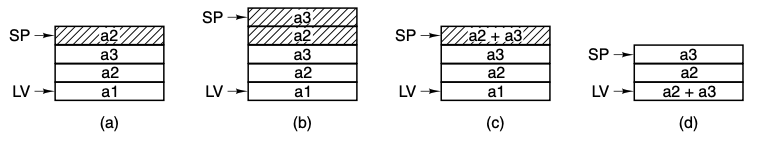
\includegraphics[width=\textwidth]{stack_add.png}
  \caption{Evoluzione dello stack durante le operazioni di somma e
    assegnazione}\label{fig:stack_add}
\end{figure}

Supponiamo che il processore si trovi al passo (c) e debba eseguire l'istruzione
\lstinline{IADD}; per farlo deve, in prima analisi:
\begin{enumerate}
  \item eseguire un primo accesso in memoria, per prelevare il primo operando;
  \item eseguire un secondo accesso in memoria, per prelevare il secondo
  operando;
  \item sommare i due operandi;
  \item eseguire un terzo accesso in memoria, per scrivere il risultato.
\end{enumerate}

Per fare questo è necessario controllare gli accessi in memoria, l'ALU, ed
eseguire delle operazioni di mantenimento (e.g.~aggiornare il puntatore alla
testa dello stack, che è modificato dalle operazioni di push e pop).

L'implementazione del processore Mic-1 che presentiamo è detta in \textit{logica
  microprogrammata}: ciascuna istruzione IJVM è implementata come una sequenza
di \textit{microistruzioni}, che complessivamente compongono il
\textit{microprogramma}, memorizzato in una ROM interna al processore. Per
capire come è strutturata una microistruzione e come è possibile realizzare un
microprograma che implementi un set di istruzioni, è necessario introdurre
anzitutto l'unità operativa del processore.

\section{L'Unità Operativa}
L'unità operativa del processore che intendiamo progettare comprende l'ALU, i
suoi ingressi e le sue uscite (tra cui i registri che si interfacciano con la
memoria), ed è mostrata in fig.~\ref{fig:datapath}.

\begin{figure}
  \centering
  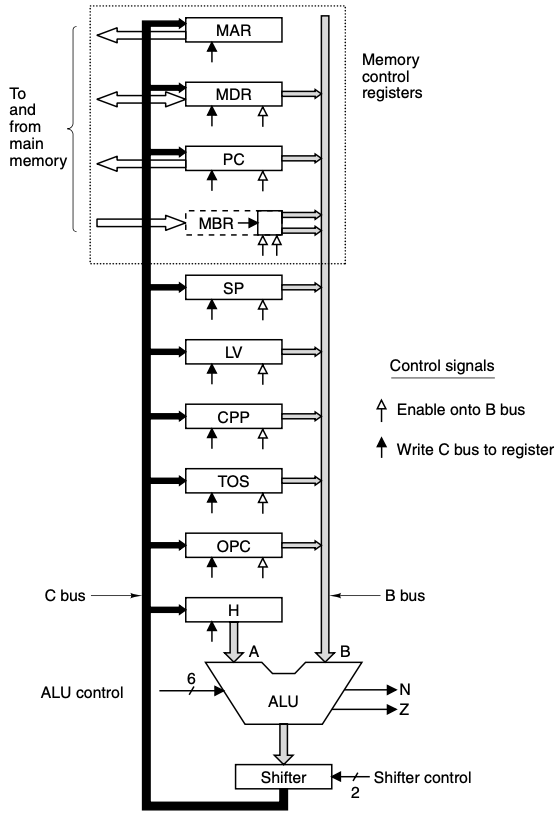
\includegraphics[width=0.9\textwidth]{datapath.png}
  \caption{Parte operativa del processore Mic-1}\label{fig:datapath}
\end{figure}

I registri hanno dimensione di 32 bit e non sono accessibili al programmatore,
ma solo al microprogramma.

\begin{mynote}{}{}
  Quando diciamo che i registri non sono accessibili al programmatore intendiamo
  che essi non fanno parte del \textit{modello di programmazione}, i.e.~non
  vengono utilizzati esplicitamente come operandi delle istruzioni. Vengono
  invece utilizzati dal microprogramma per implementare le istruzioni stesse.
\end{mynote}

L'unità operativa dispone di due bus, indicati con \lstinline{B} e
\lstinline{C}, collegati rispettivamente al secondo ingresso e all'uscita
dell'ALU; il primo ingresso dell'ALU è invece collegato esclusivamente al
registro \lstinline{H} (\textit{holding}).

Con alcune eccezioni (i cui motivi diverranno chiari a breve), i registri
dispongono di una coppia di segnali di controllo che permettono:
\begin{itemize}
    \item di abilitare il collegamento del registro al bus \lstinline{B},
    rendendolo effettivamente l'operando \lstinline{B} dell'ALU;
    \item di abilitare la scrittura sul registro del risultato fornito dall'ALU
    sul bus \lstinline{C}.
\end{itemize}

Solo un registro può essere collegato al bus \lstinline{B} in un determinato
istante, mentre il risultato dell'ALU (i.e.~il dato sul bus \lstinline{C}) può
essere scritto su più registri se necessario.

\begin{mynote}{}{}
  Il collegamento dei registri al bus \lstinline{B} può essere implementato
  usando porte tri-state o un multiplexer; nel nostro caso, useremo un
  multiplexer in quanto gli FPGA di cui facciamo uso dispongono di buffer
  tri-state esclusivamente ai pad di IO.
\end{mynote}

\subsection{L'Unità Aritmetico Logica}

L'ALU del processore Mic-1 ha due ingressi, che denominiamo \lstinline{A} e
\lstinline{B}; l'ingresso \lstinline{A} è collegato esclusivamente al registro
\lstinline{H}, mentre l'ingresso \lstinline{B} è collegato al bus
omonimo, che può essere guidato dalle nove sorgenti indicate con una freccia
grigia in fig.~\ref{fig:datapath}; le sue funzioni sono controllate mediante sei
linee di controllo, che consideriamo asserite se poste a 1:
\begin{itemize}
  \item \lstinline{F0} e \lstinline{F1} determinano l'operazione da eseguire;
  \item \lstinline{ENA} e \lstinline{ENB} abilitano singolarmente gli ingressi;
  \item \lstinline{INVA} inverte l'ingresso \lstinline{A};
  \item \lstinline{INC} incrementa di 1 il risultato.
\end{itemize}

Non tutte le combinazioni di questi segnali sono rilevanti; alcune delle più
importanti per implementare il set di istruzioni IJVM sono riportate in
tab.~\ref{fig:alu_func}.

\begin{figure}
  \centering
  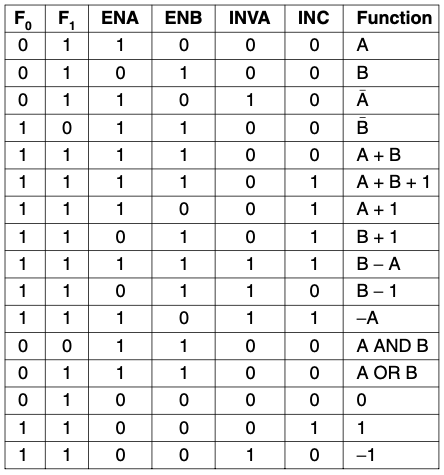
\includegraphics[width=0.7\textwidth]{alu_func.png}
  \caption{Segnali di controllo ALU e relative funzioni}\label{fig:alu_func}
\end{figure}

A questi segnali di controllo se ne aggiungono due ulteriori, utilizzati per
eseguire lo shift del risultato dell'ALU prima che esso venga posto sul bus
\lstinline{C}:
\begin{itemize}
  \item \lstinline{SLL8} (\textit{Shift Left Logical 8 bit}) esegue lo shift a
  sinistra di 8 bit, ponendo i bit meno significativi a \lstinline{0};
  \item \lstinline{SRA1} (\textit{Shift Right Arithmetic 1 bit}) esegue lo shift
  a destra di 1 bit, con estensione del segno (i.e. il bit più significativo non
  cambia).
\end{itemize}

Oltre a quella relativa al risultato, l'ALU dispone di due uscite \textit{flag}
ulteriori:
\begin{itemize}
  \item il flag \lstinline{N} è posto a 1 se il risultato è negativo;
  \item il flag \lstinline{Z} è posto a 1 se il risultato è 0.
\end{itemize}

In VHDL, l'\textit{entity declaration} per l'ALU così descritta può essere
scritta come:

\begin{myvhdl}{alu.vhd}
entity alu is
  port (
    --! ALU control
    control       : in  alu_ctrl_type;
    --! ALU operand A
    operand_a     : in  reg_data_type;
    --! ALU operand B
    operand_b     : in  reg_data_type;
    --! ALU result
    sh_result     : out reg_data_type;
    --! Negative flag
    negative_flag : out std_logic;
    --! Zero flag
    zero_flag     : out std_logic
    );
end entity alu;
\end{myvhdl}

I tipi \lstinline{alu_ctrl_type} e \lstinline{reg_data_type} non sono tipi
standard VHDL, ma sono definiti nel file \lstinline{common_defs.vhd}:

\begin{myvhdl}{common\_defs.vhd}
package common_defs is
  -- Data widths
  --! Processor register data width
  constant reg_data_width      : positive := 32;
  --! MBR register data width
  constant mbr_data_width      : positive := 8;
  --! ALU control width
  constant alu_ctrl_width      : positive := 8;

  [...]

  -- Subtypes
  --! Processor register data
  subtype reg_data_type is std_logic_vector(reg_data_width - 1 downto 0);
  --! MBR register data
  subtype mbr_data_type is std_logic_vector(mbr_data_width - 1 downto 0);
  --! ALU control type
  subtype alu_ctrl_type is std_logic_vector(alu_ctrl_width - 1 downto 0);

  [...]

end package common_defs;
\end{myvhdl}

\subsection{L'Interfaccia con la Memoria}

Il processore Mic-1 può comunicare con la memoria mediante due interfacce:
\begin{itemize}
  \item \lstinline{MAR} e \lstinline{MDR} controllano un'interfaccia
  word-addressable a 32 bit in lettura e scrittura;
  \item \lstinline{PC} e \lstinline{MBR} controllano un'interfaccia
  byte-addressable a 8 bit in sola lettura.
\end{itemize}

\begin{mynote}{}{}
  Come vedremo in seguito, la prima interfaccia è utilizzata per accedere ai
  dati su cui operano le istruzioni IJVM, rappresentati su 32 bit; la seconda,
  invece, per prelevare le istruzioni IJVM dalla memoria, che possono avere una
  lunghezza variabile in multipli di byte (e richiedono dunque più accessi
  successivi in memoria). Gli indirizzi sono comunque rappresentati su 32 bit
  per entrambe le interfacce.
\end{mynote}

Le due interfacce funzionano in modo simile in lettura: l'indirizzo da cui si
vuole leggere deve essere posto nel registro \lstinline{MAR} (\lstinline{PC});
al successivo fronte di salita del clock, il dato è disponibile nel registro
\lstinline{MDR} (\lstinline{MBR}). Indirizzano però in modo diverso la memoria:
scrivendo \lstinline{0x00000002} nel registro \lstinline{PC} e abilitando una
lettura, il byte all'indirizzo \lstinline{0x00000002} (i.e.~il byte di indirizzo
2) viene letto e posto negli 8 bit meno significativi del registro
\lstinline{MBR}; scrivendo lo stesso indirizzo nel registro \lstinline{MAR} e
abilitando una lettura, i 4 byte \lstinline{0x8}-\lstinline{0x11} (i.e.~la word
di indirizzo 2) vengono letti e posti nel registro \lstinline{MDR}.

L'interfaccia \lstinline{MAR}/\lstinline{MDR} dispone inoltre di un segnale di
\textit{write enable} (\lstinline{WE}) che, se asserito al fronte di salita di
clock, indica alla memoria di scrivere il dato contenuto in \lstinline{MDR}
all'indirizzo contenuto in \lstinline{MAR}.

\section{Le Microistruzioni}

Per controllare l'unità operativa del processore, presentata in fig.
\ref{fig:datapath}, sono necessari 29 segnali:
\begin{itemize}
    \item 9 segnali per controllare la scrittura dei dati dal bus \lstinline{C}
    ai registri;
    \item 9 segnali per controllare quale registro è collegato al bus
    \lstinline{B} e va in ingresso all'ALU;
    \item 2 segnali per abilitare lettura/scrittura sull'interfaccia
    \lstinline{MAR}/\lstinline{MDR};
    \item 1 segnale per abilitare il fetch sull'interfaccia
    \lstinline{PC}/\lstinline{MBR}.
\end{itemize}

\begin{mynote}{}{}
  Nella nostra implementazione su FPGA, i segnali di lettura per la memoria sono
  inutili in quanto i device effettivamente utilizzati non li richiedono. Sono
  stati mantenuti per compatibilità con il formato usato in~\cite{tanenbaum}.
\end{mynote}

Poiché al più un registro alla volta può essere collegato al registro
\lstinline{B}, non c'è bisogno di utilizzare effettivamente 9 segnali: dato che
al più uno di essi può essere asserito, le 10 configurazioni possibili possono
essere codificate su $\ceil{\log_{2}10} = 4$ bit.

I 24 segnali individuati permettono di controllare l'unità operativa per un
ciclo di clock; per completare una microistruzione, è necessario aggiungere due
campi aggiuntivi, che chiamiamo \lstinline{NEXT_ADDRESS} e \lstinline{JAM}, che
descriveremo approfonditamente quando parleremo dell'unità di controllo; per il
momento, è sufficiente sapere che sono necessari a determinare la
microistruzione da eseguire nel ciclo di clock successivo.

\begin{figure}
  \centering
  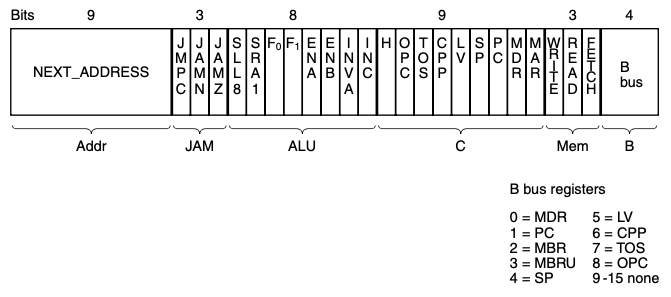
\includegraphics[width=\textwidth]{mu_instr.png}
  \caption{Il formato delle microistruzioni del Mic-1}\label{fig:mu_instr}
\end{figure}

In fig.~\ref{fig:mu_instr} è presentato il formato che adotteremo per le
microistruzioni, rappresentate su 36 bit; come anticipato, ogni microistruzione
comprende i seguenti campi:
\begin{itemize}
  \item \lstinline{Addr} - Indirizzo di una potenziale prossima microistruzione;
  \item \lstinline{JAM} - Determina come è selezionata la prossima
  microistruzione;
  \item \lstinline{ALU} - Controllo dell'ALU e dello shifter;
  \item \lstinline{C} - Controlla quali registri vengono scritti dal bus
  \lstinline{C};
  \item \lstinline{Mem} - Controlla le operazioni di memoria;
  \item \lstinline{B} - Seleziona il registro connesso al bus \lstinline{B}
  (codifica in fig.~\ref{fig:mu_instr}).
\end{itemize}

\subsection{Esempio pratico: l'istruzione \lstinline{IADD}}

Ora che abbiamo un'idea del funzionamento dell'unità operativa e della struttura
di una microistruzione, possiamo analizzare più nel dettaglio il modo in cui
viene eseguita un'istruzione IJVM. Consideriamo ad esempio l'istruzione
\lstinline{IADD}: quando l'abbiamo introdotta, abbiamo detto che ``esegue il pop
dei due elementi in cima allo stack e il push della loro somma''; questo
significa che il processore, in prima analisi, dovrebbe eseguire due accessi in
memoria in lettura, un'operazione di somma con l'ALU ed un accesso in memoria in
scrittura. In pratica, però, l'implementazione del microprogramma Mic-1 mantiene
due utili invarianti:
\begin{itemize}
  \item il registro \lstinline{SP} (\textit{Stack Pointer}), al termine dell'esecuzione
  di un'istruzione IJVM, contiene sempre l'indirizzo dell'elemento in testa allo
  stack;
  \item il registro \lstinline{TOS} (\textit{Top of Stack}), al termine dell'esecuzione
  di un'istruzione IJVM, contiene sempre il valore dell'elemento in testa allo
  stack.
\end{itemize}

È dunque sufficiente un singolo accesso in memoria, e l'istruzione può essere
eseguita in tre cicli di clock (i.e.~tre microistruzioni); supponendo che lo
stack si trovi nello stato in fig.~\ref{fig:stack_add}~(b), per quanto detto in
precedenza \lstinline{TOS} contiene il valore \lstinline{a3}; da questo stato:
\begin{enumerate}
  \item il contenuto di \lstinline{SP} viene decrementato di 1 e scritto sia in
  \lstinline{SP} che in \lstinline{MAR}, e si avvia l'operazione di lettura; si
  noti che \lstinline{SP} punta ora alla posizione da cui deve essere letto il
  valore di \lstinline{a2} e in cui in seguito sarà scritta la somma
  \lstinline{a2 + a3};
  \item il contenuto di \lstinline{TOS} è posto nel registro \lstinline{H};
  \item i dati contenuti in \lstinline{TOS} e \lstinline{MDR} (dato proveniente
  dalla memoria) sono sommati e posti sia in \lstinline{TOS} che in
  \lstinline{MDR}, si avvia una operazione di scrittura.
\end{enumerate}
È possibile verificare manualmente che queste operazioni rispettano le
invarianti enunciate in precedenza, e che il valore in cima allo stack è ora
proprio la somma dei due operandi che vi erano stati posti in precedenza.

Trascurando per ora i campi \lstinline{Addr} e \lstinline{JAM}, siamo in grado
di codificare le microistruzioni:
\begin{enumerate}
  \item
  \begin{itemize}
    \item \lstinline{ALU}: \lstinline{110110} (decremento dell'operando \lstinline{B});
    \item \lstinline{C}: \lstinline{000001001} (bus \lstinline{C} scrive su
    \lstinline{SP} e \lstinline{MAR});
    \item \lstinline{Mem}: \lstinline{010} (lettura dati);
    \item \lstinline{B}: \lstinline{0100} (\lstinline{SP} controlla il bus \lstinline{B}).
  \end{itemize}
  \item
  \begin{itemize}
    \item \lstinline{ALU}: \lstinline{010100} (l'operando \lstinline{B} passa invariato);
    \item \lstinline{C}: \lstinline{100000000} (bus \lstinline{C} scrive su
    \lstinline{H});
    \item \lstinline{Mem}: \lstinline{000} (nessuna operazione di memoria);
    \item \lstinline{B}: \lstinline{0111} (\lstinline{TOS} controlla il bus \lstinline{B}).
  \end{itemize}
  \item
  \begin{itemize}
    \item \lstinline{ALU}: \lstinline{111100} (somma degli operandi
    \lstinline{A} e \lstinline{B});
    \item \lstinline{C}: \lstinline{001000010} (bus \lstinline{C} scrive su
    \lstinline{MDR} e \lstinline{TOS});
    \item \lstinline{Mem}: \lstinline{100} (scrittura dati);
    \item \lstinline{B}: \lstinline{0000} (\lstinline{MDR} controlla il bus \lstinline{B}).
  \end{itemize}
\end{enumerate}

\section{L'Unità di Controllo}

\begin{figure}
  \centering
  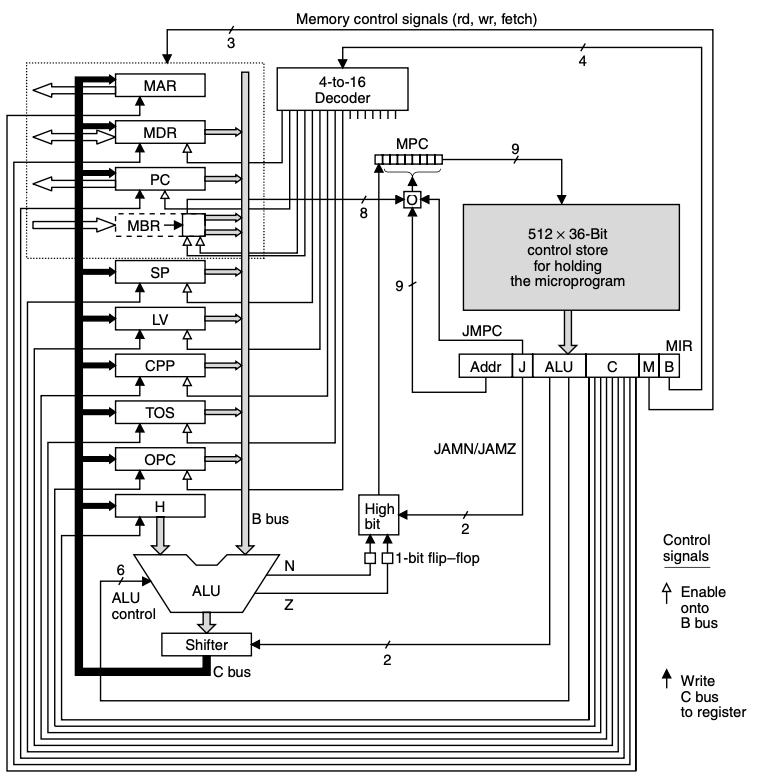
\includegraphics[width=\textwidth]{mic1.png}
  \caption{Diagramma completo del processore Mic-1}\label{fig:mic1}
\end{figure}

In fig.~\ref{fig:mic1} è riportato il diagramma completo del processore Mic-1,
in cui oltre all'unità operativa sono riportate le componenti dell'unità di
controllo.

L'unità del controllo del Mic-1 si comporta come un \textit{sequencer},
producendo in ciascun ciclo:
\begin{enumerate}
  \item lo stato dei segnali di controllo;
  \item l'indirizzo della prossima microistruzione da eseguire.
\end{enumerate}

Il microprogramma è effettivamente memorizzato in una memoria a sola lettura,
interna al processore, detta \textit{control store}; in prima analisi, il
control store contiene le microistruzioni del microprogramma allo stesso modo in
cui la memoria principale contiene le istruzioni (di livello ISA) del programma
da eseguire.

L'accesso al control store richiede infatti un'interfaccia, controllata dai due
registri \lstinline{MPC} (MicroProgram Counter) e \lstinline{MIR}
(MicroInstruction Register); non è necessario un segnale di lettura, in quanto
il control store è letto continuamente ad ogni ciclo.

Un'importante differenza è legata al fatto che, mentre le istruzioni del
programma sono eseguite generalmente in ordine sequenziale (a meno ovviamente di
istruzioni di salto), ciascuna microistruzione specifica esplicitamente
l'indirizzo della successiva.

\chapter{Il Livello ISA}

\chapter{Installazione}

\begin{commandshell}
  apt-get install ghdl
\end{commandshell}

\begin{thebibliography}{2}
  \bibitem{tanenbaum}
  Andrew S. Tanenbaum and Todd Austin.
  \textit{Structured Computer Organization}.
  Pearson, 2013.

  \bibitem{calc}
  Gianni Conte, Antonino Mazzeo, Nicola Mazzocca and Paolo Prinetto.
  \textit{Architettura dei Calcolatori}.
  CittàStudi, 2015.
\end{thebibliography}
\end{document}
